\chapter{Design of MCM and MIMO Processing Systems for Urban Communication}

This chapter focuses on the algorithms implemented as part of the \acrshort{mcm}-\acrshort{mimo} system. We look into the different aspects of transmitter block, channel parameters and receiver block of our system. We look into the simulation of \acrshort{siso}, \acrshort{simo} ( transmit \gls{spatial diversity}), \acrshort{miso} (\acrshort{ostbc}) and \acrshort{mimo} ( both \gls{spatial diversity} and multiplexing(inverse channel decoding and \acrshort{svd})).
 
\section{Basic Overview of our System}

Figure \ref{fig:general block digram} shows the general block diagram of a communication system, similar to the one mentioned in Chapter 1.
In the following sections we discuss the role of each block in detail by building on the foundation we have laid in the previous chapter.

\begin{figure}[!htbp]
\centering
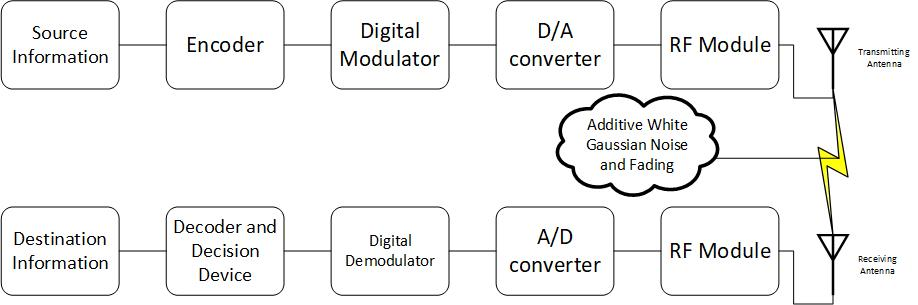
\includegraphics[scale=0.8]{Chapter 3/Figures/Wireless Communication System Block Diagram}
\label{fig:general block digram}
\caption{General Wireless Communication System Block Diagram}
\end{figure}

\section{Transmitter}

We begin by exploring the various sections of the transmitter block. We do not concern ourselves with the source information as they are just randomized binary digits generated by the \gls{matlab} rand function. Neither do we concern ourselves with the \acrlong{dac}(\acrshort{dac}) as it is beyond the scope of this report.\\

Instead, in this section we focus on the \acrshort{qam} modulator and various precoders which work on the principles explained in Chapter 2. We also look into the \acrlong{prbs}(\acrshort{prbs}) generator which is used for channel estimation and the tone loading algorithm which we employ in the cases of \acrshort{siso}, \acrshort{simo} and \acrshort{mimo} both in diversity and multiplexing cases.

\subsection{PRBS Generator}
A good \acrlong{prbs} generator is key for generating the pilot signals which is needed for the modem training phase and channel characteristic estimation. For our purposes we use the \acrshort{prbs} generator algorithm presented in \textcite{ITU2009} which is defined below.

The $n^{th}$ pseudo random binary digit $d_n$ is given by 

\begin{align*}
d_n &= 1 & \text{for n = 1 to 9}\\
d_n &= d_{n-4} \oplus d_{n-9} & \text{for n = 10 to 2 $\times$ NSC}\\
d_n &= d_{n-2 \times NSC} & \text{for n = 2 $\times$ NSC + 1 to 2 $\times$ NSC + 2}\\
d_n &= d_{4 \times NSC +2 -n} & \text{for n = 2 $\times$ NSC + 3 to 4 $\times$ NSC (n odd)}\\
d_n &= 1 \oplus d_{4 \times NSC +4 -n} & \text{for n = 2 $\times$ NSC + 3 to 4 $\times$ NSC (n even)}
\end{align*}
Here \acrshort{nsc} is the total number of subcarriers, taken to be 256 in our case. Hence, we can generate upto 1024 \acrshort{prbs} digits. However, we limit ourselves to the first 512 digits only.

\subsection{Tone Loading Algorithm for the transmitter}
Once we have determined the channel conditions by transmitting the pilot signals and measured the \acrshort{snr} of each subchannel to create a channel profile, it becomes necessary to load the data bits onto these subchannels in an efficient manner. Common sense tells us that the subchannels with higher \acrshort{snr} should carry more bits than those with lower \acrshort{snr}. We show through our algorithm that this is indeed the case.\\
The basis for our tone loading algorithm is the capacity law given by Shannon in \textcite{Shannnon1948}. Using this formula, we determine the number of bits that a given subchannel can support for it's given \acrshort{snr}. Then, we round the number of bits and calculate the power deviation thus obtained by applying the inverse of the capacity law. As long as this deviation is within the agreed upon threshold, we add and remove bits between the subchannels until a stable tone loading situation arises.\\
The limit we have set for our purposes is $\pm 2$ dB and we have added the additional constraint of setting the maximum number of bits for any channel to be 20. The exact details of the algorithm is given in Algorithm \ref{alg:Fine Gains Algorithm}.

\begin{algorithm}[!htbp]
\caption{Fine Gains Tone Loading Algorithm}
\label{alg:Fine Gains Algorithm}
\begin{algorithmic}
\STATE {$b_i \gets log_2(1+SNR_i)$}\\
\STATE {$\hat{b}_i \gets \nint{b_i}$}\\
\STATE {$\delta_i \gets b_i - \hat{b}_i$}\\
\STATE {$P_{\delta_i} \gets 3 \times \delta_i$}\\
\STATE {$P_{\delta_{total}} \gets \sum_{i=1}^{NSC} P_{\delta_i}$}\\
\WHILE {$P_{\delta_{total}} > P_{threshold} \OR P_{\delta_{total}} < -P_{threshold}$}
	\IF {$P_{\delta_{total}} > P_{threshold}$}
		\STATE {$position=\verb|POS|(\verb|MAX|(\delta_i))$}\\
		\STATE {$\hat{b}_{position} \gets \hat{b}_{position} - 1 $}\\
		\STATE {$\delta_{position} \gets b_{position} - \hat{b}_{position}$}\\
		\STATE {$P_{\delta_{position}} \gets 3 \times \delta_{position}$}\\
		\STATE {$P_{\delta_{total}} \gets \sum_{i=1}^{NSC} P_{\delta_i}$}\\
	\ELSIF {$P_{\delta_{total}} < -P_{threshold}$}
		\STATE {$position=\verb|POS|(\verb|MIN|(\delta_i))$}\\
		\STATE {$\hat{b}_{position} \gets \hat{b}_{position} + 1 $}\\
		\STATE {$\delta_{position} \gets b_{position} - \hat{b}_{position}$}\\
		\STATE {$P_{\delta_{position}} \gets 3 \times \delta_{position}$}\\
		\STATE {$P_{\delta_{total}} \gets \sum_{i=1}^{NSC} P_{\delta_i}$}\\
	\ENDIF
\ENDWHILE
\STATE {$SNR_i \gets 2^{\hat{b}_i}-1$} 
\end{algorithmic}
\end{algorithm}

\subsection{QAM Modulator}
Among the various modulation schemes available for us, we chose the \acrshort{qam} modulation technique because it is extremely power efficient and also maintains a good degree of spectral efficiency.\\

One of the problems we run into with \acrshort{qam} modulation is the fact that we need to maintain large symbol constellations, especially when we are dealing with higher order \acrshort{qam} modulation schemes. Therefore, in this section we describe a fast recursive algorithm that can generate large symbol constellations by keeping only a few small constellations in memory. This approach reduces the cost of hardware required by reducing the memory elements required but still maintains a high degree of speed. The details of this are given in \ref{alg:Working of Modulator}

\begin{algorithm}[!htbp]
\caption{Bits to Constellation Mapping Algorithm}
\label{alg:Working of Modulator}
\begin{algorithmic}
\STATE {$LUT \gets \verb|{QAM_1, QAM_2, QAM_3, QAM_5}|$}
\STATE {$matrix_{transform} \gets \verb|{0, -2i, 2, 2+2i}|$}
\STATE {$i \gets 1$}
\WHILE {$i < NSC $}
	\STATE {$flag_{recursion} \gets \FALSE$}
	\IF {$b_i == 1$}
		\STATE {$symbol_i \gets \verb|QAM_1|(bits_i)$}
	\ELSIF {$b_i \% 2 == 0 \quad \AND \quad b_i \quad \NOT = 0$}
		\STATE {$bits_{extracted} \gets$ extract $bits$ into groups of 2}
		\STATE {$bits_{decimal} \gets \texttt{DEC}(bits_{extracted})$}
		\STATE {$symbol_i \gets \verb|QAM_2|(bits_{decimal})$}
		\STATE {$flag_{recursion} \gets \TRUE$}
	\ELSIF {$b_i \% 2 == 1$}
		\STATE {$symbol_i \gets \verb|QAM_3|(bits_i)$}
		\IF {$b_i > 3$}
			\STATE {$bits_{extracted} \gets$ Extract bits into groups of 2}
			\STATE{$bits_{decimal} \gets \texttt{DEC}({bits_{extracted}})$}
			\IF {$bits_{decimal} < 4$}
				\STATE {$symbol_i \gets \verb|QAM_3|(bits_{decimal})$}
			\ELSE
				\STATE {$symbol_i \gets \verb|QAM_5|(bits_{decimal})$}
			\ENDIF
			\STATE{$flag_{recursion} \gets \TRUE$}
		\ENDIF
	\ENDIF
	\IF {$flag_{recursion}$}
		\STATE {$count = 2$}
		\WHILE {$count < \texttt{SIZE}(bits_{decimal})$}
			\STATE {$bits_{decimal_{extracted}} \gets $ Extract the bits individually}
			\STATE {$point_{quadrant} \gets \texttt{GET BASIC QUADRANT POINT}$}
			\STATE {$offset \gets \texttt{FIND OFFSET(}point_{quadrant} , bits_{decimal_{extracted}})$}
			\STATE {$symbol_i \gets 2 \times symbol_i - \verb|QAM_2|(bits_{decimal_{extracted}}) + point_{quadrant} + offset$}
			\STATE {$count \gets count + 1$}
		\ENDWHILE
	\ENDIF
	\STATE {$i \gets i +1$}
\ENDWHILE
\end{algorithmic}
\end{algorithm} 




\section{Channel Parameters}
In the previous section, we discussed the transmitter portion of our system, now we look into the channel parameters which are mostly randomized in nature. The various channel parameters like noise, fading and path loss are discussed in the following paragraphs.

\subsection{AWGN Noise}
All communication is affected by noise, we have assumed \acrlong{awgn} noise as the noise function of choice. To generate this, we have used the \gls{matlab} function \emph{randn} which generates a Gaussian function with mean as $0$ and variance as $1$. Then we multiply this function with the noise variance of our choice to get the noise signal. Mathematically, \acrshort{awgn} function is given by 
\begin{align*}
noise&= \frac{1}{\sqrt{2\pi\sigma^2}}e^{\frac{x^2}{2\sigma^2}}
\end{align*}

Where $\sigma$ is the noise variance or power. In \gls{matlab}, this is given by the statement
\begin{verbatim}
noise = sqrt(noise_power_abs/2) .* ((randn(Nsc,1)) + 1i*randn(Nsc,1));
\end{verbatim}
Here, \acrshort{nsc} is the \acrlong{nsc}. Since we are trying to add noise to all the subchannels, the vector is of the size $\acrshort{nsc} \times 1$.

\subsection{Rayleigh Fading}
In the previous chapter we mentioned fading in wireless channels. We also mentioned that \gls{rayleigh fading} was the model of choice for our report. \gls{rayleigh fading} is viewed as a reasonable model for tropospheric and ionospheric propagation as well as for heavy urban settings for wireless signals. \gls{rayleigh fading} is most applicable when there is no dominant propagation along a line of sight between the transmitter and receiver. \gls{rayleigh fading} is any function that varies as per the Rayleigh distribution which is the radial component of the sum of two uncorrelated Gaussian random variables. In \gls{matlab} this is generated through,
\begin{verbatim}
rayleigh_channel = sqrt(1/2) .* (randn(1) + 1i*randn(1))
\end{verbatim}
where the two \emph{randn} functions produce the two uncorrelated Gaussian functions.

\subsection{Path Loss Function}
Path loss function determine the way in which the transmitted signal degrades with distance before the signal reaches the receiver. Since we are focused on \acrlong{los} path propagation we consider \acrshort{los} path loss formulation as given by Friis Transmission formula.
\begin{align*}
P_r &= \frac{P_t G_t G_r \lambda^2}{(4 \pi r)^2} 
\end{align*}
where:

\begin{align*}
P_r &= \text{Received Signal Power}\\
P_t &= \text{Transmitted Signal Power, in our simulations it is 1 mW}\\
G_t &= \text{Transmitter Antenna Gain, in our simulations it is 8}\\
G_r &= \text{Receiver Antenna Gain, in our simulation it is 1}\\
r &= \text{Distance of separation between the two antennas, in our simulations it is 1 Km}\\
\lambda &= \text{Wavelength of the signal wave}.\\
\end{align*}


\section{Receiver}
The receiver we have employed in our system consists of an estimator, decoder and demodulator. The estimator uses the principle of maximum likelihood estimation. In \acrshort{mli} at the receiver we take the received symbol and plot it as a point on the symbol constellation. Then, we calculate the Euclidian distance of this point from all the constellation points and select the constellation point whose Euclidian distance is closest to our received symbol point. This technique is optimal and gives us the least amount of error thereby improving our system performance.\\

The decoders like Alamouti decoder and \acrshort{svd} decoder have already been discussed in the previous chapter.

Our estimator system also works on a similar principle but makes use of the unique constellation mapping algorithm to greatly simplify the decision making process by following Algorithm \ref{alg:Working of Estimator}.\\

Once the estimator has estimated a constellation point for us, the demodulator converts this constellation point into the binary digits representing the constellation point. Similar to the case of modulation, we do not have all the constellations stored in memory but generate them dynamically using a recursive algorithm. This process is shown in Algorithm \ref{alg:Working of Demodulator} 

\begin{algorithm}[!htbp]
\caption{Estimation Algorithm}
\label{alg:Working of Estimator}
\begin{algorithmic}
\STATE {$LUT \gets \verb|{QAM_1, QAM_2, QAM_3}|$} 
\STATE {$i \gets 1$}
\WHILE {$i < NSC $}
	\IF {$b_i == 0$}
		\STATE {$estimate_i \gets 0$}
	\ELSIF {$b_i == 1$}
		\STATE {$estimate_i \gets \verb|CLOSEST|(\verb|QAM1|, received_i)$}
	\ELSIF {$b_i == 3$}
		\STATE {$estimate_i \gets \verb|CLOSEST|(\verb|QAM_3|, received_i)$}
	\ELSIF {$b_i \geq 2$}
		\STATE {$real_i \gets \floor{\texttt{REAL}(received_i)}$}
		\STATE {$imag_i \gets \floor{\texttt{IMAG}(received_i)}$}
		\IF{$real_i \% 2 ==0$}
			\STATE {$real_i = real_i +1$}
		\ENDIF
		\IF{$imag_i \% 2 ==0$}
			\STATE {$imag_i = imag_i +1$}
		\ENDIF
		\STATE {$estimate_i \gets real_i + imag_i$}
		\STATE {$estimate_i \gets \verb|BOUND TO MAX|(estimate_i)$} 
	\ENDIF
	\STATE {$i \gets i +1$}
\ENDWHILE
\end{algorithmic}
\end{algorithm} 

\begin{algorithm}[!htbp]
\caption{Constellation to Bits Mapping Algorithm}
\label{alg:Working of Demodulator}
\begin{algorithmic}
\STATE {$LUT \gets \verb|{QAM_1, QAM_2, QAM_3, QAM_5}|$}
\STATE {$matrix_{transform} \gets \verb|{0, -2i, 2, 2+2i}|$}
\STATE {$i \gets 1$}
\WHILE {$i < NSC $}
	\IF {$b_i == 1$}
		\STATE {$symbol_i \gets \texttt{BIN(FIND}(estimate_i, \verb|QAM_1|))$}
	\ELSIF {$b_i == 3$}
		\STATE {$symbol_i \gets \texttt{BIN(FIND}(estimate_i, \verb|QAM_3|))$}
	\ELSIF {$b_i \geq 2$}
		\STATE {$symbol_i \gets \texttt{NULL}$}
		\IF {$b_i \% 2 == 0$}
			\STATE {$limit \gets \frac{b_i}{2} -1$}
		\ELSE
			\STATE {$limit \gets \frac{b_i-3}{2} -1$}
		\ENDIF
		\STATE {$point_{quadrant} \gets \texttt{GET BASIC QUADRANT POINT}$}
		\STATE{$count \gets 1$}
		\WHILE{$count < limit$}
			\STATE{$offset \gets \texttt{FIND OFFSET(}point_{quadrant} , estimate_i)$}
			\STATE {$value_{binary} \gets \texttt{BIN(FIND(}offset, matrix_{transform}))$}
			\STATE {$symbol_i \gets symbol_i + value_{binary}$}
			\STATE{$estimate_i \gets \frac{estimate_i}{2}$}
			\STATE{$count \gets count +1$}
		\ENDWHILE
	\ENDIF
	\STATE {$i \gets i +1$}
\ENDWHILE
\end{algorithmic}
\end{algorithm} 



\section{Operation of the System in Different Modes}
In this section we demonstrate the various modes in which our system can be operated. The algorithm that the system follows in each mode is described in detail in this section. In some cases like \acrshort{mimo} it is possible to operate the system with various precoders and hence we discuss in detail these algorithms as well.

\subsection{SISO Mode}
In the \acrlong{siso} mode, only one antenna each is present at both the transmitter and receiver. The steps involved in sending the data from transmitter to the receiver in the \acrshort{siso} is given in Algorithm \ref{alg:Operation in SISO Mode}.

\begin{algorithm}[!htbp]
\caption{Operation in SISO Mode}
\label{alg:Operation in SISO Mode}
\begin{enumerate}
\item Get pilot signals through the PRBS Generator
\item Get QAM symbols by modulating the pilot bits with the modulator
\item Obtain the Rayleigh channel coefficient
\item Obtain the received power with the help of LOS function
\item Generate the noise signal
\item Determine the channel coefficient as $h \gets \sqrt{\frac{P_r}{P_t}} \times rayleigh$
\item Send the pilot signals from transmitter to the receiver
\item Get the received pilot symbols by doing $symbol_{received} \gets symbol_{sent} \times h$
\item Estimate the \acrshort{snr} of the subchannels with the help received power
\item Estimate the value of channel coefficients at the receiver with the help of received pilot signals
\item Get the data bits and modulate them into \acrshort{qam} symbols
\item Perform tone loading with the help of fine gains algorithm
\item Send the data \acrshort{qam} symbols as per the tone loading profile
\item Add noise signal and multiply data signal with channel coefficients to simulate path loss and fading
\item Demodulate the received data symbols with the help of estimated channel coefficients at the receiver
\item Use a \acrlong{mli} to determine the sent bits
\item Calculate the \acrshort{ber} for the system
\end{enumerate}
\end{algorithm} 


\subsection{SIMO System}
In the \acrlong{simo} mode, only one antenna is present at the transmitter but there are 2 antennas at the receiver leading to 2 possible antenna paths. The steps involved in sending the data from transmitter to the receiver in the \acrshort{simo} is given in Algorithm \ref{alg:Operation in SIMO Mode}.

\begin{algorithm}[!htbp]
\caption{Operation in SIMO Mode}
\label{alg:Operation in SIMO Mode}
\begin{enumerate}
\item Get pilot signals through the PRBS Generator
\item Get QAM symbols by modulating the pilot bits with the modulator
\item Obtain both the Rayleigh channel coefficient
\item Obtain the received power with the help of LOS function for both paths
\item Generate the noise signal
\item Determine both the channel coefficients as $h_i \gets \sqrt{\frac{P_{r_i}}{P_{t_i}}} \times rayleigh_i$
\item Send the pilot signals from transmitter to the receiver in both paths
\item Get the received pilot symbols for both paths by doing $symbol_{received} \gets symbol_{sent} \times h_i$
\item Estimate the \acrshort{snr} of the subchannels for both paths with the help received power
\item Estimate the value of channel coefficients for both paths at the receiver with the help of received pilot signals
\item For each subchannel choose the optimal antenna path between the two possibilities
\item Get the data bits and modulate them into \acrshort{qam} symbols
\item Perform tone loading with the help of fine gains algorithm for the optimal data paths
\item Send the data \acrshort{qam} symbols as per the tone loading profile in the optimal data paths
\item Add noise signal and multiply data signal with respective channel coefficient to simulate path loss and fading
\item Demodulate the received data symbols with the help of estimated channel coefficient of the path in which data was received at the receiver
\item Use a \acrlong{mli} to determine the sent bits
\item Calculate the \acrshort{ber} for the system
\end{enumerate}
\end{algorithm} 

\subsection{MISO System}
In the \acrlong{miso} mode, only one antenna is present at the receiver but there are 2 antennas at the transmitter leading to 2 possible antenna paths. The steps involved in sending the data from transmitter to the receiver in the \acrshort{miso} is given in Algorithm \ref{alg:Operation in MISO Mode}.

\begin{algorithm}[!htbp]
\caption{Operation in MISO Mode}
\label{alg:Operation in MISO Mode}
\begin{enumerate}
\item Get pilot signals through the PRBS Generator
\item Get QAM symbols by modulating the pilot bits with the modulator
\item Obtain both the Rayleigh channel coefficient
\item Obtain the received power with the help of LOS function for both paths
\item Generate the noise signal
\item Determine both the channel coefficients as $h_i \gets \sqrt{\frac{P_{r_i}}{P_{t_i}}} \times rayleigh_i$
\item Send the pilot signals from transmitter to the receiver in both paths
\item Get the received pilot symbols for both paths by doing $symbol_{received} \gets symbol_{sent} \times h_i$
\item Estimate the value of channel coefficients for both paths at the receiver with the help of received pilot signals
\item Get the data bits and modulate them into \acrshort{qam} symbols
\item Perform Alamouti Coding and send the data symbol and the conjugate data symbol in alternate cycles and alternate paths as described in Alamouti Coding Scheme
\item Add noise signal and multiply data signal with respective channel coefficient to simulate path loss and fading
\item Demodulate the received data symbols with the help of estimated channel coefficient of the path in which data was received at the receiver
\item Perform Alamouti decoding as previously described to get 2 data symbols in 2 consecutive cycles
\item Use a \acrlong{mli} to determine the sent bits
\item Calculate the \acrshort{ber} for the system
\end{enumerate}
\end{algorithm} 

\subsection{MIMO System}
In the \acrlong{mimo} mode, 2 antennas are present at both the receiver and the transmitter leading to 4 possible antenna paths. This also affords us the option of whether we want to use the system in diversity mode or multiplexing mode depending on the channel conditions.\\
If the channel we are operating in has low \acrshort{snr} characteristics, we go ahead and operate in the diversity mode. The steps involved in sending the data from transmitter to the receiver in the \acrshort{mimo} diversity mode is given in Algorithm \ref{alg:Operation in MIMO Diversity Mode}.\\
However, supposing we have a sufficiently high \acrshort{snr}, we can then operate in the multiplexing mode. The steps involved in operating the system in \acrshort{mimo} multiplexing mode are given in Algorithm \ref{alg:Operation in MIMO Multiplexing Mode}.\\

For the multiplexing mode again, we have different precoding options like Inverse Channel Estimation Precoding and \acrlong{svd} precoding. These techniques have already been discussed in the previous chapter and we provide the algorithm for implementation here. Algorithm \ref{alg:Operation in MIMO Inverse Channel Estimation Mode} provides the details of operating the system with an Inverse Channel Estimator and Algorithm \ref{alg:Operation in MIMO SVD Mode} provides the details for operating the system with a \acrshort{svd} precoder.\\

\begin{algorithm}[!htbp]
\caption{Operation in MIMO Diversity Mode}
\label{alg:Operation in MIMO Diversity Mode}
\begin{enumerate}
\item Get pilot signals through the PRBS Generator
\item Get QAM symbols by modulating the pilot bits with the modulator
\item Obtain all the Rayleigh channel coefficients
\item Obtain the received power with the help of LOS function for all  paths
\item Generate the noise signal
\item Determine all the channel coefficients as $h_i \gets \sqrt{\frac{P_{r_i}}{P_{t_i}}} \times rayleigh_i$
\item Send the pilot signals from transmitter to the receiver in all paths
\item Get the received pilot symbols for all paths by doing $symbol_{received} \gets symbol_{sent} \times h_i$
\item Estimate the \acrshort{snr} of the subchannels with the help received power
\item Estimate the value of channel coefficients for all paths at the receiver with the help of received pilot signals
\item For each subchannel choose the optimal antenna path between the four possibilities
\item Get the data bits and modulate them into \acrshort{qam} symbols
\item Perform tone loading with the help of fine gains algorithm for the optimal data paths
\item Add noise signal and multiply data signal with respective channel coefficient to simulate path loss and fading
\item Demodulate the received data symbols with the help of estimated channel coefficient of the path in which data was received at the receiver
\item Use a \acrlong{mli} to determine the sent bits
\item Calculate the \acrshort{ber} for the system
\end{enumerate}
\end{algorithm} 

\begin{algorithm}[!htbp]
\caption{Operation in MIMO Multiplexing Mode}
\label{alg:Operation in MIMO Multiplexing Mode}
\begin{enumerate}
\item Get pilot signals through the PRBS Generator
\item Get QAM symbols by modulating the pilot bits with the modulator
\item Obtain all the Rayleigh channel coefficients
\item Obtain the received power with the help of LOS function for all  paths
\item Generate the noise signal
\item Determine all the channel coefficients as $h_i \gets \sqrt{\frac{P_{r_i}}{P_{t_i}}} \times rayleigh_i$
\item Send the pilot signals from transmitter to the receiver in all paths
\item Get the received pilot symbols for all paths by doing $symbol_{received} \gets symbol_{sent} \times h_i$
\item Estimate the \acrshort{snr} of the subchannels with the help received power
\item Estimate the value of channel coefficients for all paths at the receiver with the help of received pilot signals
\item For transmitting antenna $T_1$ choose the optimal channel path from the two available paths. Similarly, for $T_2$ choose an optimal path from the two available paths.
\item Get the data bits and modulate them into \acrshort{qam} symbols
\item Perform tone loading for $T_1$ and $T_2$ onto their respective optimal channels with the help of fine gains algorithm
\item Add noise signal and multiply data signal with respective channel coefficient to simulate path loss and fading
\item Demodulate the received data symbols with the help of estimated channel coefficient of the path in which data was received at the receiver
\item Use a \acrlong{mli} to determine the sent bits
\item Calculate the \acrshort{ber} for the system
\end{enumerate}
\end{algorithm}

\begin{algorithm}[!htbp]
\caption{Operation in MIMO Multiplexing Mode with Inverse Channel Estimation Precoding}
\label{alg:Operation in MIMO Inverse Channel Estimation Mode}
\begin{enumerate}
\item Get pilot signals through the PRBS Generator
\item Get QAM symbols by modulating the pilot bits with the modulator
\item Obtain all the Rayleigh channel coefficients
\item Obtain the received power with the help of LOS function for all  paths
\item Generate the noise signal
\item Determine all the channel coefficients as $h_i \gets \sqrt{\frac{P_{r_i}}{P_{t_i}}} \times rayleigh_i$
\item Send the pilot signals from transmitter to the receiver in all paths
\item Get the received pilot symbols for all paths by doing $symbol_{received} \gets symbol_{sent} \times h_i$
\item Estimate the value of channel coefficients for all paths at the receiver with the help of received pilot signals
\item Obtain the inverse of the channel coefficient matrix
\item Get the data bits and modulate them into \acrshort{qam} symbols
\item Precode the data bits being sent with the inverse of the channel coefficient matrix
\item Add noise signal and multiply data signal with respective channel coefficient to simulate path loss and fading
\item Demodulate the received data symbols with the help of estimated channel coefficient of the path in which data was received at the receiver. Since we are precoding with the inverse channel matrix, the channel effects nullify the precoding and there is no need for a decoder.
\item Use a \acrlong{mli} to determine the sent bits
\item Calculate the \acrshort{ber} for the system
\end{enumerate}
\end{algorithm}

\begin{algorithm}[!htbp]
\caption{Operation in MIMO Multiplexing Mode with SVD Precoding}
\label{alg:Operation in MIMO SVD Mode}
\begin{enumerate}
\item Get pilot signals through the PRBS Generator
\item Get QAM symbols by modulating the pilot bits with the modulator
\item Obtain all the Rayleigh channel coefficients
\item Obtain the received power with the help of LOS function for all  paths
\item Generate the noise signal
\item Determine all the channel coefficients as $h_i \gets \sqrt{\frac{P_{r_i}}{P_{t_i}}} \times rayleigh_i$
\item Send the pilot signals from transmitter to the receiver in all paths
\item Get the received pilot symbols for all paths by doing $symbol_{received} \gets symbol_{sent} \times h_i$
\item Estimate the value of channel coefficients for all paths at the receiver with the help of received pilot signals
\item Obtain the \acrlong{svd} of the channel coefficient matrix by doing $[U \Sigma V] \gets \verb|SVD|(\begin{bmatrix} h \end{bmatrix}$
\item Get the data bits and modulate them into \acrshort{qam} symbols
\item Precode the data bits being sent by doing $symbols_{precoded} \gets symbols_{sent} \times \begin{bmatrix} V \end{bmatrix}$
\item Add noise signal and multiply data signal with respective channel coefficient to simulate path loss and fading
\item Demodulate the received data symbols with the help of estimated channel coefficient of the path in which data was received at the receiver.
\item Decode the data bits received by doing $symbols_{decoded} \gets symbols_{received} \times \begin{bmatrix} U \end{bmatrix}$
\item Use a \acrlong{mli} to determine the sent bits
\item Calculate the \acrshort{ber} for the system
\end{enumerate}
\end{algorithm}

\section*{Summary}
In this chapter we saw the details of the implementation of the entire system. We also studied some of the algorithms we developed to help us achieve optimal system performance like the fine gains algorithm and the dynamic constellation mapping algorithm. In the next section we will see the system performance for the different modes and compare the performance across various modes.

